\section{Solução Implementada}

    O aplicativo Encontre na UFMS foi desenvolvido com o intuito de facilitar a navegação pelo campus da UFMS em Campo Grande, permitindo que usuários encontrem e localizem pontos de interesse dentro do campus, estes sendo cadastrados por outros usuários, possibilitando que locais que não estão presentes em outros aplicativos de localização sejam documentados e compartilhados com a comunidade acadêmica. Os usuários também terão poder de avaliar os locais cadastrados, podendo assim, ajudar outros usuários a escolherem o melhor local para suas necessidades.

\subsection{Análise Crítica e contribuição do Encontre na UFMS}
    Para podermos analisar o diferencial do aplicativo Encontre na UFMS podemos compará-lo com os aplicativos Google Maps e Localização UFMS. O Google Maps é um aplicativo de geolocalização muito utilizado no mundo todo, porém, ele não é focado em um local específico, como o campus da UFMS, e sim em todo o mundo, sendo assim ele não possui registrado diversos locais de menor escala mas que podem ser de grande importância para algum visitante ou alunos. Já o Localização UFMS é um aplicativo web que disponibiliza um mapa interativo da UFMS que possui mais de 2900 pontos de interesse registrados, porém, ele não possui alguns pontos de interesse que podem ser de grande importância para a comunidade acadêmica, como por exemplo, o Restaurante Universitário e também não informa ao usuário como chegar até o local desejado já que ele é focado em apenas mostrar informações sobre um certo local, ele também não tem fotos de todos os locais e não é colaborativo uma vez que apenas a administração da UFMS pode adicionar novos locais.

\subsection{Comparação entre o Encontre na UFMS e outros aplicativos}
\begin{table}[h]
    \begin{tabularx}{\textwidth}{|X|X|X|X|}
        \hline
        \textbf{Características} & \textbf{Google Maps} & \textbf{Localização UFMS} & \textbf{Encontre na UFMS} \\ \hline
        \textbf{Objetivo Principal} & Geolocalização global & Mapa interativo da UFMS & Navegação pelo campus da UFMS \\ \hline
        \textbf{Público-Alvo} & Usuários em geral & Comunidade acadêmica da UFMS & Comunidade acadêmica da UFMS \\ \hline
        \textbf{Principais Funcionalidades} & Busca de locais, rotas, informações de contato, horários de funcionamento & Busca de locais no campus, informações sobre pontos de interesse & Busca de locais, rotas, cadastro colaborativo de locais, avaliações de locais \\ \hline
    \end{tabularx}
    \caption{Comparação entre aplicativos de localização}
    \footnotesize  \centering{\textbf{Fonte: Autor original}}
    \label{tab:comparacao-aplicativos}
\end{table}

\subsection{Implementação}

    O desenvolvimento do aplicativo Encontre na UFMS foi dividido em duas partes principais: o backend e o frontend. Trataremos a seguir de cada uma dessas partes, detalhando as tecnologias utilizadas e as funcionalidades implementadas.

\subsubsection{Frontend}

    O frontend foi desenvolvido utilizando o framework Flutter, que permite o desenvolvimento de aplicativos móveis para Android e iOS a partir de um único código fonte. O Flutter é uma ferramenta moderna e de fácil utilização, que permite a criação de interfaces de usuário atraentes e responsivas.

    O código foi desenvolvido com base na \textit{Clean Architecture}, que é um padrão de arquitetura de software que visa separar as responsabilidades do código em camadas bem definidas, facilitando a manutenção e a evolução do sistema. A arquitetura do aplicativo foi dividida em três camadas principais: a camada de apresentação, a camada de domínio e a camada de dados. A camada de apresentação é responsável por exibir os dados para o usuário e capturar as interações do usuário com o sistema. A camada de domínio contém as regras de negócio do sistema, enquanto a camada de dados é responsável por acessar os dados do sistema, seja de um banco de dados local ou de uma API remota.

    \begin{figure}[h]
        \centering
        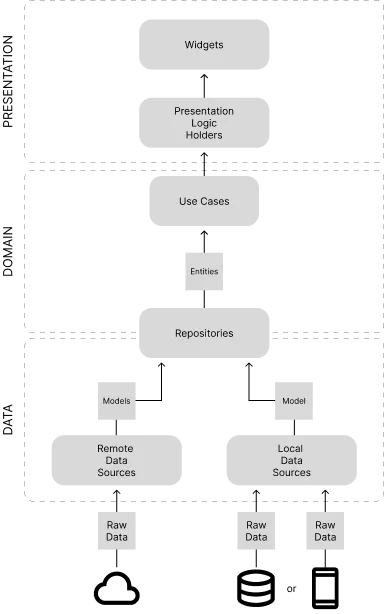
\includegraphics[width=55mm,height=80mm]{imagens/cleanarch.png}
        \caption{\scriptsize Clean Architecture}
        \footnotesize  \centering{\textbf{Fonte: X}}
        \label{fig:clean-architecture}
    \end{figure}

    Embora o Flutter seja capaz de gerar aplicativos nativos para Android e iOS, o aplicativo Encontre na UFMS foi desenvolvido apenas para Android, visto que a Apple, dona do sistema operacional iOS, restringe o desenvolvimento para seu sistema caso o desenvolvedor não possua um dispositivo da marca. Mas, em teoria, o aplicativo poderia ser facilmente adaptado para iOS, bastando apenas compilar o código fonte em um ambiente de desenvolvimento da Apple.

\subsubsection{Backend}

    O backend foi desenvolvido utilizando o framework Fastify, a fim de garantir excelente desempenho em velocidade e segurança, possuindo uma arquitetura escalável, sendo programado em Typescript para melhor definição de variáveis e classes durante o desenvolvimento, evitando eventuais erros que poderiam ser causados por incompatibilidade de tipos.

\subsection{Testes e Execução}

    O aplicativo Encontre na UFMS foi testado em diversos dispositivos Android, a fim de garantir a compatibilidade e o bom funcionamento em diferentes tamanhos de tela e versões do sistema operacional. Foi utilizado o emulador do Android Studio para testar o aplicativo no Pixel 6a na API 33 do Android mas foi principalmente testado em dispositivos físicos, como o Galaxy S21 fe, pela facilidade de uso e para poder verificar a usabilidade real do aplicativo em todo momento.

\subsubsection{Diagrama de Navegação}

    O diagrama de navegação do aplicativo apresentado na Figura 2 demonstra os fluxos básicos de navegação que o usuário pode experenciar
    durante o uso do mesmo, vale destacar que algumas telas como Perfil e Criação só são acessíveis caso o usuário esteja logado.

    \begin{figure}[h]
        \centering
        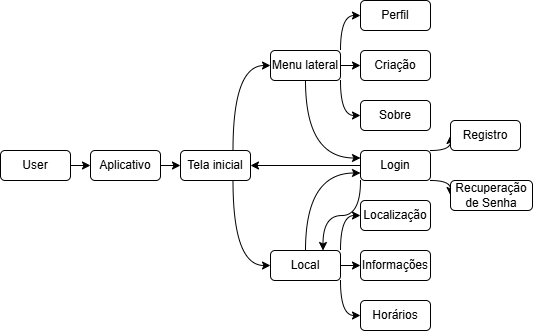
\includegraphics[width=120mm,height=70mm]{imagens/navegacao.png}
        \caption{\scriptsize Diagrama de Navegação}
        \footnotesize  \centering{\textbf{Fonte: Autor original}}
        \label{fig:diagrama-navegacao}
    \end{figure}